% small.tex
\documentclass[12pt]{beamer}
\usetheme{amcg}
\beamertemplatenavigationsymbolsempty
\renewcommand{\thefootnote}{}
\providecommand{\e}[1]{\ensuremath{\times 10^{#1}}}
\usepackage{mathptmx}
\usepackage{helvet}
\newcommand\TILDE{\char`\~}
\usepackage{listings}

% items enclosed in square brackets are optional; explanation below
\title[Diamond]{Using Diamond}
\subtitle[]{}
\institute{}
\author[Christian Jacobs]{\large{Christian Jacobs}}
\date{}


\begin{document}


%--- the titlepage frame -------------------------%
\begin{frame}
  \titlepage
\end{frame}


\section{Diamond}

\begin{frame}
    \frametitle{Context}
\begin{itemize}
    \item To run a simulation in Fluidity, we need to give it some \textbf{input}. For example:
    \begin{itemize}
      \item The path to the mesh file
      \item What fields we want to solve for
      \item Initial conditions, boundary conditions
      \item What spatial and temporal discretisations will be used
      \item Solver settings
    \end{itemize}
    \item All of these need to be \textbf{specified by the user in a file}, which is then given to Fluidity.
    \item This is where \textbf{Diamond} comes in...
\end{itemize}
\end{frame}

\begin{frame}
    \frametitle{Diamond and FLML}
\begin{itemize}
    \item Diamond is an XML editor, used to \textbf{create/edit simulation configuration files}.
    \item These files have a ``.flml'' (FLuidity Markup Language) file extension, but are basically XML files with elements pre-defined...
    \item ...in another XML file called a \textbf{schema}. Schemas contain all the available options that the user can choose from, and act like a \textbf{blueprint} or \textbf{template} from which .flml files can be derived.
    \newline
    \item Diamond loads the schema and gives you all the options contained within.
\end{itemize}
\end{frame}

\begin{frame}
    \frametitle{Diamond's User Interface}
\begin{center} 
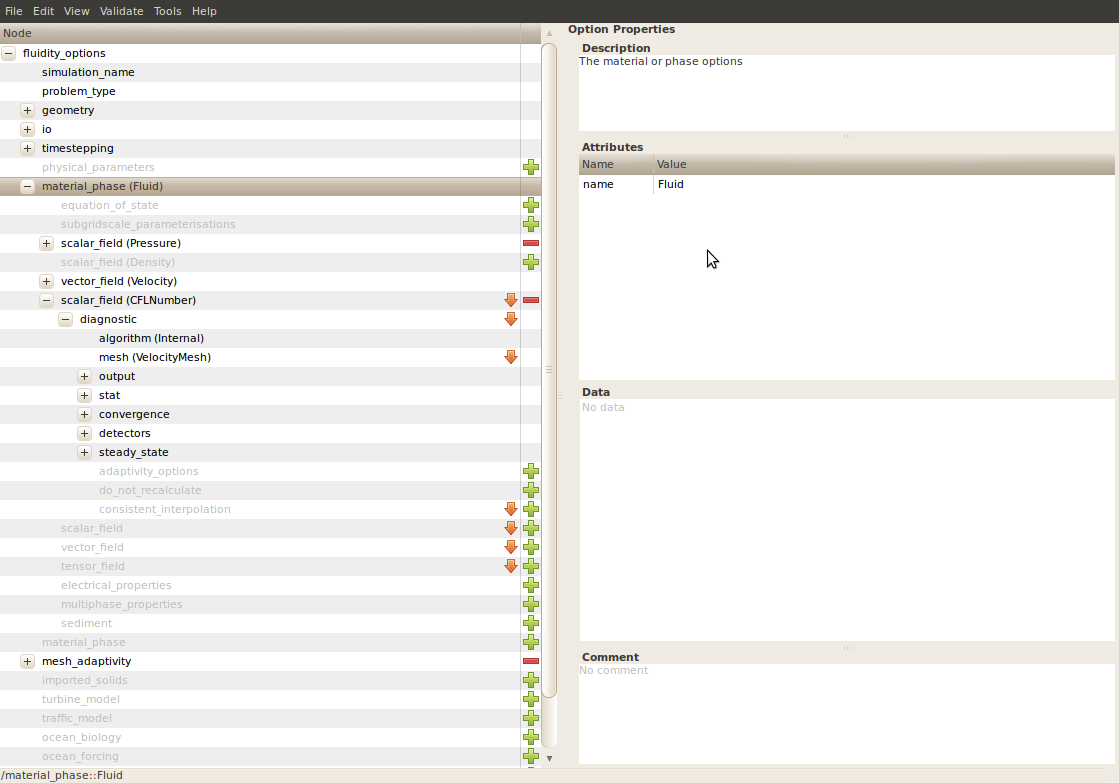
\includegraphics[width=0.75\textwidth]{images/diamond.png} 
\end{center} 
\footnotetext{Ham et al., 2010}
\end{frame}

\begin{frame}
    \frametitle{Live demo}
\begin{itemize}
    \item Stommel gyre
    \item Prescribed velocity
    \item Adaptive mesh
    \item Advect a tracer (temperature) and measure mixing
\end{itemize}
\end{frame}

\begin{frame}
    \frametitle{Output}
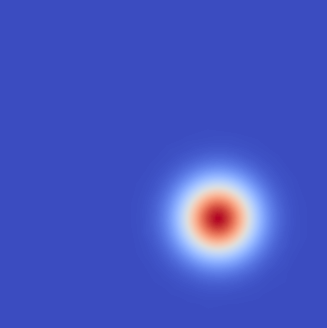
\includegraphics[width=0.48\textwidth]{images/stommel_0.png}
\hspace{1mm}
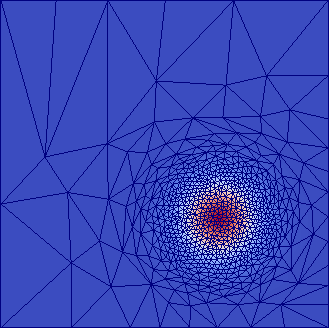
\includegraphics[width=0.48\textwidth]{images/stommel_0_mesh.png}
\end{frame}
\begin{frame}
    \frametitle{Output}

\includegraphics[width=0.48\textwidth]{images/stommel_7.png}
\hspace{1mm}
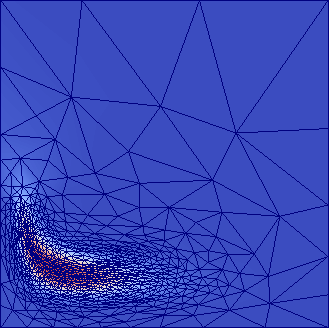
\includegraphics[width=0.48\textwidth]{images/stommel_7_mesh.png}
\end{frame}
\begin{frame}
    \frametitle{Output}
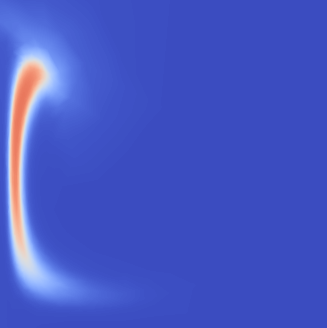
\includegraphics[width=0.48\textwidth]{images/stommel_10.png}
\hspace{1mm}
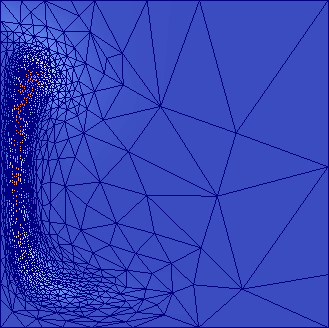
\includegraphics[width=0.48\textwidth]{images/stommel_10_mesh.png}
\end{frame}
\begin{frame}
    \frametitle{Output}
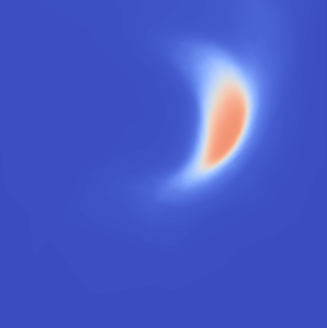
\includegraphics[width=0.48\textwidth]{images/stommel_20.png}
\hspace{1mm}
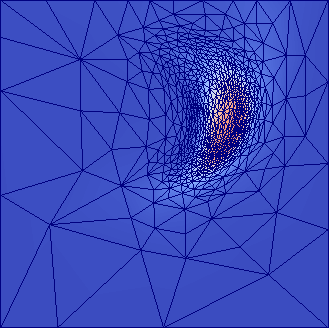
\includegraphics[width=0.48\textwidth]{images/stommel_20_mesh.png}
\end{frame}

\begin{frame}
    \frametitle{Before we start...}

Make a directory in your data/$<$username$>$ directory: \texttt{mkdir stommel}
\\
\texttt{cd stommel}
\\
\texttt{cp /scratch/Stommel2\_adapt.* .}
\\
\texttt{cp /scratch/stommel.pvsm .}
\\
\texttt{cp /scratch/Stommel\_function.py .}

\end{frame}


\begin{frame}
    \frametitle{Create a FLML}
Live demo

\texttt{diamond -s /data/<username>/fluidity/schema/fluidity\_options.rng my.flml}
\end{frame}

\begin{frame}
    \frametitle{Running Fluidity}
\scriptsize{\texttt{/path/bin/fluidity my.flml}}
\\
\scriptsize{\texttt{/data/<username>/fluidity/bin/fluidity my.flml}}
\\
\scriptsize{\texttt{/home/<username>/fluidity/bin/fluidity -l -v2 my.flml}}
\end{frame}


\begin{frame}
	\frametitle{Visualising your output}
\begin{columns}
\begin{column}{0.6\textwidth}

\texttt{paraview -{}-state=stommel.pvsm}
\end{column}
\begin{column}{0.4\textwidth}
\begin{center}
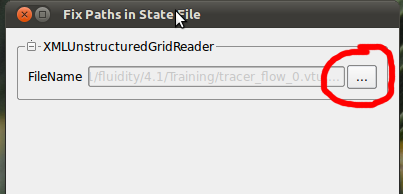
\includegraphics[width=0.9\textwidth]{images/State_box.png}

\vspace{2mm}

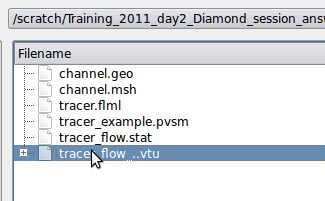
\includegraphics[width=\textwidth]{images/State_Open.png}
\end{center}
\end{column}
\end{columns}


\end{frame}


\end{document}

